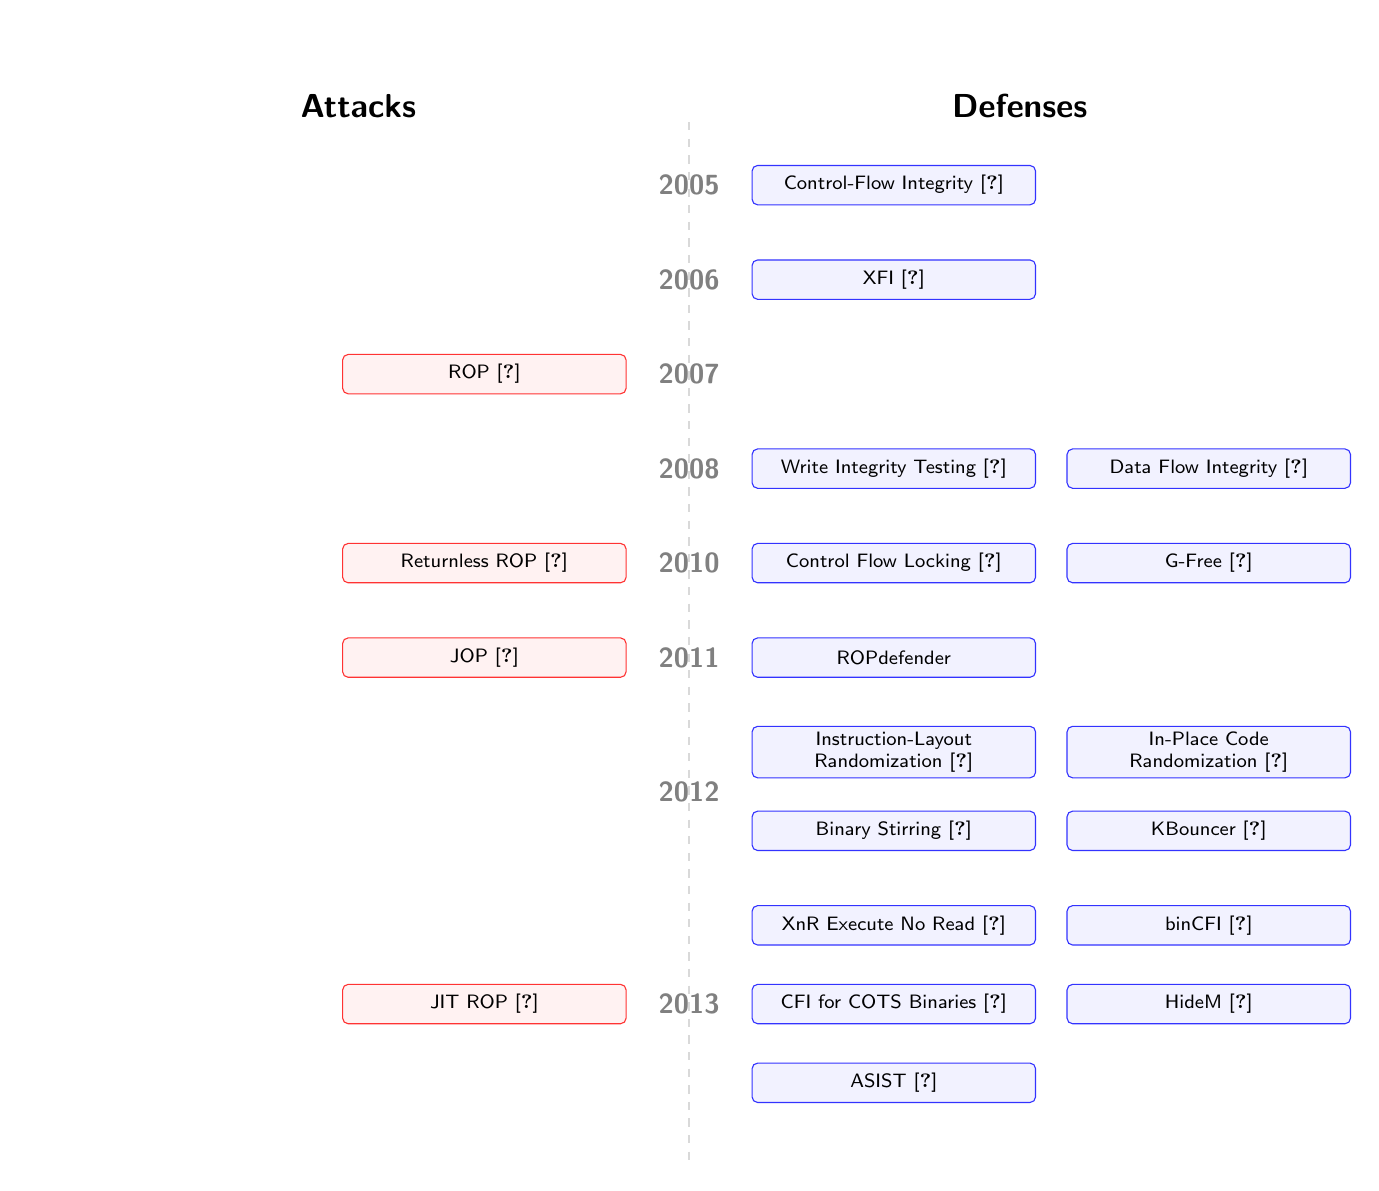
\begin{tikzpicture}[year node/.style={font=\bfseries\sffamily\color{gray}, align=center, inner sep=2pt},attack node/.style={draw=red!80, fill=red!5, rounded corners=2pt, font=\scriptsize\sffamily, align=center, minimum width=3.60cm, minimum height=0.5cm, inner sep=2pt, text width=3.40cm, execute at begin node=\setlength{\emergencystretch}{0pt}\tolerance 200\hyphenpenalty 10000\exhyphenpenalty 10000},defense node/.style={draw=blue!80, fill=blue!5, rounded corners=2pt, font=\scriptsize\sffamily, align=center, minimum width=3.60cm, minimum height=0.5cm, inner sep=2pt, text width=3.40cm, execute at begin node=\setlength{\emergencystretch}{0pt}\tolerance 200\hyphenpenalty 10000\exhyphenpenalty 10000},spine/.style={thick, gray!30, dashed}]%
\node[font=\large\bfseries\sffamily] at (-4.2,1.0) {Attacks};%
\node[font=\large\bfseries\sffamily] at (4.2,1.0) {Defenses};%
  % Year 2005%
\node[year node] at (0.0,0.0) {2005};%
\node[defense node] at (2.6,0.0) {Control{-}Flow Integrity \allowbreak\cite{Abadi2005}};%
  % Year 2006%
\node[year node] at (0.0,-1.2) {2006};%
\node[defense node] at (2.6,-1.2) {XFI \allowbreak\cite{Erlingsson2006}};%
  % Year 2007%
\node[year node] at (0.0,-2.4) {2007};%
\node[attack node] at (-2.6,-2.4) {ROP \allowbreak\cite{Shacham2007}};%
  % Year 2008%
\node[year node] at (0.0,-3.6) {2008};%
\node[defense node] at (2.6,-3.6) {Write Integrity Testing \allowbreak\cite{Akritidis2008}};%
\node[defense node] at (6.6,-3.6) {Data Flow Integrity \allowbreak\cite{castro2006}};%
  % Year 2010%
\node[year node] at (0.0,-4.8) {2010};%
\node[attack node] at (-2.6,-4.8) {Returnless ROP \allowbreak\cite{checkoway2010}};%
\node[defense node] at (2.6,-4.8) {Control Flow Locking \allowbreak\cite{Bletsch2011b}};%
\node[defense node] at (6.6,-4.8) {G{-}Free \allowbreak\cite{Onarlioglu2010}};%
  % Year 2011%
\node[year node] at (0.0,-6.0) {2011};%
\node[attack node] at (-2.6,-6.0) {JOP \allowbreak\cite{Bletsch2011a}};%
\node[defense node] at (2.6,-6.0) {ROPdefender};%
  % Year 2012%
\node[year node] at (0.0,-7.7) {2012};%
\node[defense node] at (2.6,-7.2) {Instruction{-}Layout\\ Randomization \allowbreak\cite{Hiser2012}};%
\node[defense node] at (6.6,-7.2) {In{-}Place Code\\ Randomization \allowbreak\cite{Pappas2012a}};%
\node[defense node] at (2.6,-8.2) {Binary Stirring \allowbreak\cite{Wartell2012}};%
\node[defense node] at (6.6,-8.2) {KBouncer \allowbreak\cite{Pappas2013b}};%
  % Year 2013%
\node[year node] at (0.0,-10.4) {2013};%
\node[attack node] at (-2.6,-10.4) {JIT ROP \allowbreak\cite{Snow2013}};%
\node[defense node] at (2.6,-9.4) {XnR Execute No Read \allowbreak\cite{Backes2013}};%
\node[defense node] at (6.6,-9.4) {binCFI \allowbreak\cite{zhang2013}};%
\node[defense node] at (2.6,-10.4) {CFI for COTS Binaries \allowbreak\cite{zhang2013}};%
\node[defense node] at (6.6,-10.4) {HideM \allowbreak\cite{Goktas2016b}};%
\node[defense node] at (2.6,-11.4) {ASIST \allowbreak\cite{papadogiannakis2013}};%
\path[spine,draw] (0.0,0.8) -- (0.0,-12.4);%
\path[use as bounding box] (-8.40,-12.40) rectangle (8.40,2.00);%
\end{tikzpicture}